\subsection{Iterators}

\begin{frame}[fragile]{Idea}
    For an array:
    \begin{cpp}
for (int i = 0; i != n; ++i)
  do_something(a[i]);
    \end{cpp}
    For a \ttt{vector} or a \ttt{string}:
    \begin{cpp}
for (std::size_t i = 0; i != c.size(); ++i)
  do_something(c[i]);
    \end{cpp}
    For a linked-list?
    \pause
    \begin{cpp}
for (Node *p = l.head; p; p = p->next)
  do_something(p->value);
    \end{cpp}
\end{frame}

\begin{frame}{Idea}
    \begin{figure}[h]
        \centering
        \begin{minipage}{0.48\textwidth}
            \centering
            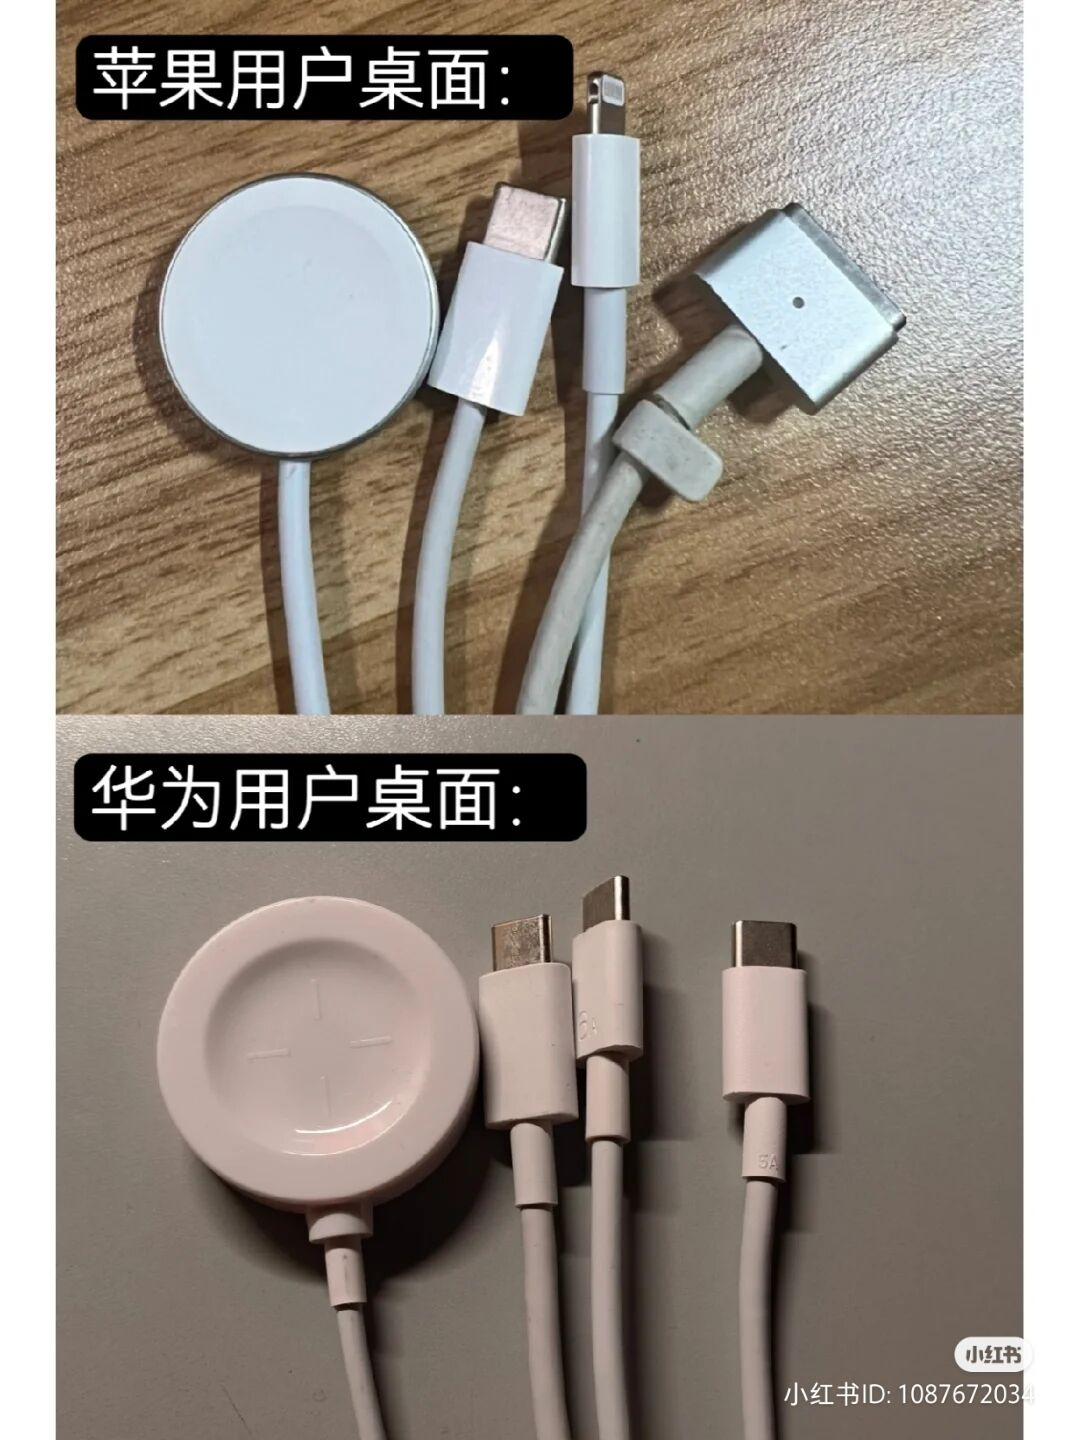
\includegraphics[scale=0.135]{figures/interface1.jpg}
        \end{minipage}
        \begin{minipage}{0.48\textwidth}
            \centering
            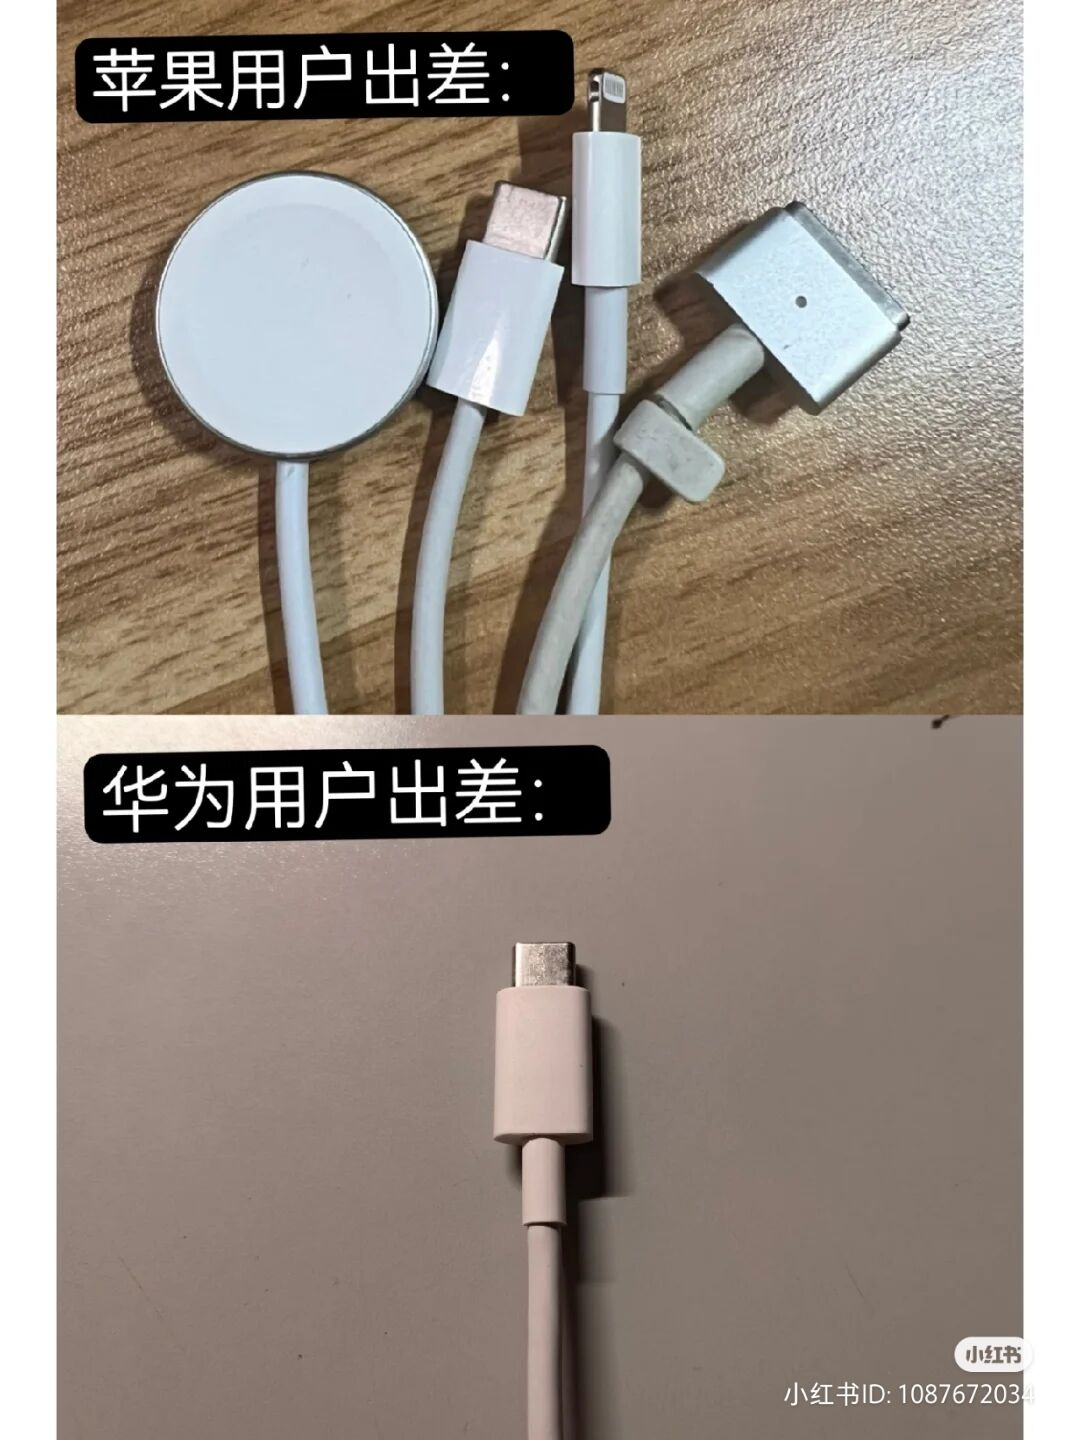
\includegraphics[scale=0.135]{figures/interface2.jpg}
        \end{minipage}
    \end{figure}
\end{frame}

\begin{frame}[fragile]{Using Iterators}
    \begin{cpp}
std::vector<int> v = {2, 3, 5, 7, 11, 13};
for (auto it = v.begin(); it != v.end(); ++it)
  *it = *it * *it;
for (auto it = v.begin(); it != v.end(); ++it)
  std::cout << *it << " ";
std::cout << std::endl;
    \end{cpp}
    \begin{itemize}
        \item The type of `\ttt{it}' is \ttt{std::vector<int>::iterator}.
        \item \ttt{v.begin()} returns the iterator pointing to the first element.
        \item \ttt{v.end()} returns the \textbf{off-the-end} iterator, positioned ``one past the end'' of the container.
        \item If the container is empty, we have \ttt{v.begin() == v.end()}.
    \end{itemize}
\end{frame}

\begin{frame}[fragile]{Iterator Operations}
    The iterator of every container supports these operations:
    \begin{center}
        \begin{tabular}{|ll|}
            \hline
            \begin{cpp}
*iter
            \end{cpp} & \footnotesize Returns reference to the element denoted by \ttt{iter}.\\
            \begin{cpp}
iter->mem
            \end{cpp} & \footnotesize Equivalent to \ttt{(*iter).mem}.\\
            \begin{cpp}
++iter
            \end{cpp} & \footnotesize Increments \ttt{iter} to refer to the next element in the container.\\
            \begin{cpp}
iter++
            \end{cpp} & \footnotesize Postfix version. Returns the copy of the original iterator.\\
            \begin{cpp}
==, !=
            \end{cpp} & \footnotesize Equal iff both iterators are pointing to the same position.\\
            \hline
        \end{tabular}
    \end{center}
    \begin{itemize}
        \item Dereferencing or incrementing an off-the-end iterator is undefined behavior.
    \end{itemize}
\end{frame}

\begin{frame}[fragile]{Examples}
    Count the number of upper-case letters and convert them to lower-case.
    \pause
    \begin{cpp}
int upper_cnt = 0;
for (auto it = s.begin(); it != s.end(); ++it) {
  if (std::isupper(*it)) {
    ++upper_cnt;
    *it = std::tolower(*it);
  }
}
    \end{cpp}
    \pause
    Convert the first word to upper-case.
    \pause
    \begin{cpp}
for (auto it = s.begin();
    it != s.end() && !std::isspace(*it); ++it)
  *it = std::toupper(*it);
    \end{cpp}
\end{frame}

\begin{frame}[fragile]{Range-\bluett{for}}
    The range-based \bluett{for} loop is treated as traversing using iterators.
    \begin{cpp}
for (auto x : v)
  do_something(x);
// Equivalent:
for (auto it = v.begin(); it != v.end(); ++it) {
  auto x = *it;
  do_something(x);
}
    \end{cpp}
\end{frame}

\begin{frame}[fragile]{Range-\bluett{for}}
    \begin{cpp}
for (const auto &x : v)
  do_something(x);
// Equivalent:
for (auto it = v.begin(); it != v.end(); ++it) {
  const auto &x = *it;
  do_something(x);
}
    \end{cpp}
    \pause
    \begin{itemize}
        \item Any object that could be traversed using the range-\bluett{for} loop must provide \ttt{begin()} and \ttt{end()}, which return an iterator that supports
        \begin{itemize}
            \item \bluett{operator*}: dereference
            \item \bluett{operator++}: prefix increment
            \item \bluett{operator!=}
        \end{itemize}
    \end{itemize}
\end{frame}

\begin{frame}[fragile]{\ttt{const\_iterator}}
    On a \const object, \ttt{begin()} and \ttt{end()} return a different iterator type:
    \begin{cpp}
inline void print_vector(const std::vector<int> &v) {
  for (auto it = v.begin(); it != v.end(); ++it)
    std::cout << *it << " ";
  std::cout << std::endl;
}
    \end{cpp}
    \begin{itemize}
        \item \ttt{it} here is of type \ttt{vector<int>::const\_iterator}.
        \item Dereferencing \ttt{it} returns a reference-to-\bluett{const}, which is not modifiable.
        \item Since C++11, we have explicit way to obtain \ttt{const\_iterator}s: The \ttt{cbegin()} and \ttt{cend()} member functions.
    \end{itemize}
\end{frame}

\begin{frame}[fragile]{Other Iterator Operations}
    Operations Supported by \ttt{vector} and \ttt{string} iterators:
    \begin{center}
        \begin{tabular}{|ll|}
            \hline
            \begin{cpp}
iter + n
            \end{cpp} & \footnotesize Returns an iterator positioned \ttt{n} elements forward.\\
            \begin{cpp}
iter - n
            \end{cpp} & \footnotesize Returns an iterator positioned \ttt{n} elements backward.\\
            \begin{cpp}
n + iter
            \end{cpp} & \footnotesize Equivalent to \ttt{iter + n}.\\
            \begin{cpp}
iter += n
            \end{cpp} & \footnotesize Equivalent to \ttt{iter = iter + n}.\\
            \begin{cpp}
iter -= n
            \end{cpp} & \footnotesize Equivalent to \ttt{iter = iter - n}.\\
            \begin{cpp}
iter1 - iter2
            \end{cpp} & \footnotesize Returns the distance between two iterators.\\
            \begin{cpp}
<,<=,>,>=
            \end{cpp} & \footnotesize Relational operators.\\
            \hline
        \end{tabular}
    \end{center}
    \begin{itemize}
        \item The return-type of \ttt{iter1 - iter2} is a \textbf{type-alias member} named \ttt{difference\_type}. e.g. \ttt{string::difference\_type}. It is a signed integer type.
        \item \ttt{iter1 - iter2} returns the number that when added to \ttt{iter2} yields \ttt{iter1}.
    \end{itemize}
\end{frame}

\begin{frame}[fragile]{Relational Operators of Iterators}
    \ttt{<, <=, >, >=}: comparing the positions of two iterators in the container.
    \begin{itemize}
        \item If they are not positioned in the same container, the result is undefined.
        \item Why did I always use \ttt{!=} in the \bluett{for} loops?
        \pause
        \begin{itemize}
            \item Not all kinds of iterators support \ttt{<, <=, >, >=}, but all of them support \ttt{==} and \ttt{!=}.
        \end{itemize}
    \end{itemize}
\end{frame}